\label{app_design}
Antes de empezar el proceso de desarrollo se han tomado una serie de decisiones de diseño. Realizar este paso ayuda a tener una mejor idea de lo que se quiere hacer, cuales serán las necesidades y qué problemas pueden surgir. En este capítulo se describirá el diseño de la aplicación incluyendo los cambios que se han realizado durante el desarrollo.

%\section{Estructura del programa}
\section{Núcleo, incialización y gestión de inputs}
\label{world}
El elemento más importante de la aplicación, alrededor del cual girará el resto, es la clase ``World". Puede entenderse esta clase como la ``puerta de entrada" del flujo del motor hacia la aplicación. Es la primera clase de la aplicación en llamarse en la incialización, actualización y finalización del programa (véase el apartado \ref{fps_bucle_ejecucion} sobre el bucle de ejecución).

Desde ``World" se incializa la cámara, y las luces. Un fichero externo \texttt{.json} describe el estado inicial de la aplicación y a partir de esta configuración se inicializa el progrma. También es la primera clase de la aplicación en recibir la orden de actualización del motor y los inputs del usario y debe transmitirsela a los diferentes elementos que gestione.

También se encargará de actualizar en cada iteración los diferentes componentes de la aplicación, y gestionar los estados del sistema de estados (explicado en el apartado \ref{state_pattern}).

%%%%%%%%%%%%%%%%%%%%%%%%%%%%%%%%%%%%%%%%%%%%%%%%%%%%%%%%%%%%%%%%%%%%%%%%%%%%%
%%%%%%%%%%%%%%%%%%%%%%%%%%%%%%%%%%%%%%%%%%%%%%%%%%%%%%%%%%%%%%%%%%%%%%%%%%%%%
%%%%%%%%%%%%%%%%%%%%%%%%%%%%%%%%%%%%%%%%%%%%%%%%%%%%%%%%%%%%%%%%%%%%%%%%%%%%%

\section{Gestión y generación de entidades}
\label{managers}

Como se ha explicado en la sección \ref{engine_design}, la aplicación se comunica con el motor a través de la escena y las entidades. Un primer punto importante es mantener el control de dichas entidades para que no acaben esparcidas por el código.

\subsection{Managers y generadores}
Normalmente es suficiente con organizar las entidades en estructuras de datos dentro de la propia clase World (\ref{world}). Sin embargo, algunos casos específicos como las paredes y huecos (cuya generación se explica en el apartado \ref{walls_holes} o los interiores), son lo suficientemente complejos y numerosos como para tener su propio gestor.

Dentro cada gestor hay una o varias listas de elementos que se organizan según sus índices en la lista, y que se inicializan con un tamaño predefinido. Se ha decidido hacer de este modo para evitar que la lista cambie de tamaño constantemente, provocando reinicializaciones de memoria. Una consecuencia es que debe hacerse una estimación del número de elementos que habrá y controlar mediante aserciones que no se supere ese número. 

Como las paredes se definen en forma de conjuntos de paredes, para referirse a ellas se utilizan dos números enteros: la posición en la que empieza la primera pared y el número de paredes en el conjunto. Si cambia el tamaño de un conjunto de paredes al actualizarlo se reorganiza la lista de paredes para que no haya fragmentación, y se controla en todo momento el número de paredes en uso, puesto que el tamaño de las listas no varía nunca y leer datos no utilizados provocaría errores.

En el caso de elementos que sean atómicos, como las ventanas o los interiores, es suficiente con controlarlos con su índice.

Para evitar que desde fuera del gestor se manipulen los índices, y para tener un identificador más sencillo de manejar, los gestores crean sus propios identificadores en forma de número entero y los relacionan con los elementos de los arrays mediante mapas. Esto permite por ejemplo, que si la posición de una pared cambia (porque se ha borrado una pared anterior) su identificador externo, el que tiene el usuario, siga significando lo mismo. Si se utilizaran índices cambiar el orden de los elementos resultaría en índices incorrectos, de este modo se evita que externamente haya que preocuparse por ello. El sistema es muy similar al que se describe en el apartado \ref{manta_id_management} sobre la gestión de identificadores del motor Manta.

Aunque no es estrictamente necesario, los gestores de entidades están pensados para utilizarse a través del gestor de comandos \ref{command_pattern}.

%%%%%%%%%%%%%%%%%%%%%%%%%%%%%%%%%%%%%%%%%%%%%%%%%%%%%%%%%%%%%%%%%%%%%%%%%%%%%
%%%%%%%%%%%%%%%%%%%%%%%%%%%%%%%%%%%%%%%%%%%%%%%%%%%%%%%%%%%%%%%%%%%%%%%%%%%%%
%%%%%%%%%%%%%%%%%%%%%%%%%%%%%%%%%%%%%%%%%%%%%%%%%%%%%%%%%%%%%%%%%%%%%%%%%%%%%

\subsection{Generación de paredes}
\label{wall_gen_design}
El primer paso ha sido crear una definición de los datos que se recibirán para describir cómo ha de ser la pared. Se trata de una lista de puntos en dos dimensiones y un valor booleano que indica si esta lista debe cerrarse conectando el último punto con el primero. Esto último es importante porque, como se puede ver en la figura \ref{fig:vertical_view_walls}, la geometría de una esquina ``suelta" es diferente a la de una esquina que conecta dos paredes entre sí.

\begin{figure}[h]
    \centering
    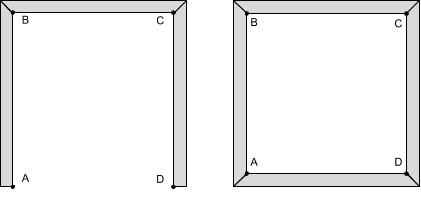
\includegraphics[width=0.65\linewidth]{Vista_Vertical_Paredes}
    \caption{Paredes en vista vertical.}
    \label{fig:vertical_view_walls}
\end{figure}

Estos datos nos permiten no sólo crear habitaciones sino también paredes únicas o incluso otros tipos de estructuras, normalmente interiores, similares a una pared. La intención es que en el futuro el programa pueda utilizarse en otras herramientas para hacer diseños más complicados como el plano de una planta completa de un edificio.

Teniendo en cuenta la estructura de una malla, explicada en el apartado \ref{mesh_light_cam}, en la figura \ref{fig:io_generatewalls} se puede ver la conversión de los datos que se espera conseguir.

\begin{figure}[H]
    \centering
    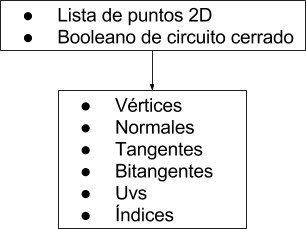
\includegraphics[width=0.5\linewidth]{IO_paredes}
    \caption{Input y output del generador de paredes.}
    \label{fig:io_generatewalls}
\end{figure}

El output está formado por listas de valores planos. Por ejemplo, la lista de vértices está formada por los valores de posición ``x,y,z" de cada uno sucesivamente.

%%%%%%%%%%%%%%%%%%%%%%%%%%%%%%%%%%%%%%%%%%%%%%%%%%%%%%%%%%%%%%%%%%%%%%%%%%%%%
%%%%%%%%%%%%%%%%%%%%%%%%%%%%%%%%%%%%%%%%%%%%%%%%%%%%%%%%%%%%%%%%%%%%%%%%%%%%%
%%%%%%%%%%%%%%%%%%%%%%%%%%%%%%%%%%%%%%%%%%%%%%%%%%%%%%%%%%%%%%%%%%%%%%%%%%%%%

\subsection{Nomenclatura de los vértices}
\label{nomenclatura_vertices}
Para referir a cada uno de los vértices se ha definido la nomenclatura ``A, B, A2, B2" como puede verse en la figura \ref{fig:nomenclatura_vertices}, además de los correspondientes ``AH, BH, A2H, B2H" en la parte alta de la pared. Posteriormente, los índices de la pared se extraen de los que habría normalmente en un cubo, aprovechando que sus vértices se conectan del mismo modo.

\begin{figure}[H]
    \centering
    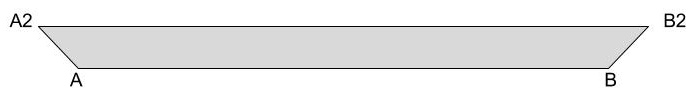
\includegraphics[width=0.75\linewidth]{Nomenclaturas_vertices}
    \caption{Nomenclatura básica de los vértices.}
    \label{fig:nomenclatura_vertices}
\end{figure}

%%%%%%%%%%%%%%%%%%%%%%%%%%%%%%%%%%%%%%%%%%%%%%%%%%%%%%%%%%%%%%%%%%%%%%%%%%%%%
%%%%%%%%%%%%%%%%%%%%%%%%%%%%%%%%%%%%%%%%%%%%%%%%%%%%%%%%%%%%%%%%%%%%%%%%%%%%%
%%%%%%%%%%%%%%%%%%%%%%%%%%%%%%%%%%%%%%%%%%%%%%%%%%%%%%%%%%%%%%%%%%%%%%%%%%%%%

\subsection{Generación de huecos}
\label{holes_design}
El siguiente paso es implementar la posibilidad de añadir puertas y ventanas a la estancia. Insertar el modelo correspondiente en cada caso no será un problema, pero para que el efecto sea convincente es necesario poder ver a través de estos. Eso implica que se debe que modificar la geometría de las paredes para que incluya huecos donde tengan que ir dichas ventanas y puertas.

Del mismo modo que con las paredes inicialmente, se define un input: por cada hueco existe un punto 3D (que como se verá a continuación, no necesariamente debe colisionar con una pared), una altura y un ancho. El input/output del algoritmo completo para generar paredes quedaría como se puede ver en la figura \ref{fig:io_generatewindows}.

\begin{figure}[H]
    \centering
    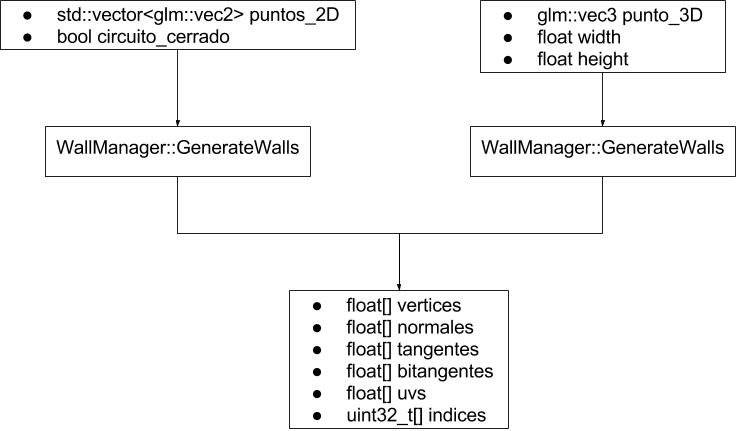
\includegraphics[width=0.75\linewidth]{I_O_ventanas}
    \caption{Nuevo input y output de GenerateWalls, incluyendo ventanas.}
    \label{fig:io_generatewindows}
\end{figure}

Para empezar a introducir huecos en las paredes, estas se deben adaptar previamente. Es conveniente que la generación de ventanas se limite a trabajar sobre un solo plano, de modo que se eliminarán los planos anterior y posterior de la pared para añadirlos después con la nueva geometría. Aunque intuitivamente pueda parecer que esto supone simplificar la geometría respecto a lo que se ha hecho hasta ahora, en realidad se complica sensiblemente. Los planos anterior y posterior de la pared van a ser siempre idénticos, pero el plano posterior es algo más alargado debido a la geometría de las esquinas que se puede apreciar en la figura \ref{fig:nomenclatura_vertices}.

\begin{figure}[H]
    \centering
    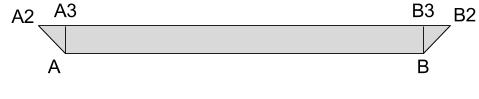
\includegraphics[width=0.75\linewidth]{Nomenclaturas_vertices_2}
    \caption{Nomenclatura final de los vértices.}
    \label{fig:nomenclatura_vertices_2}
\end{figure}

Se trata de una segunda iteración de lo visto en el apartado \ref{nomenclatura_vertices}. Con la nueva geometría las paredes se convierten en dos prismas triangulares unidos por dos planos superior e inferior de la pared. Con esto se consigue que los planos anterior y posterior que ahora le faltan a la pared sean totalmente idénticos aunque con las normales invertidas.

Todas las ventanas o puertas han de ser necesariamente rectangulares. Esta es una precondición que se ha impuesto desde desarrollo para simplificar el cálculo de los agujeros, dado que es más sencillo incorporar geometrías más complejas incluyendo paredes falsas dentro del modelo de la ventana o puerta. Por ejemplo, si en algún momento se deseara incorporar una ventana redonda, sería más sencillo incluir 4 esquinas de pared a la ventana permitiendo que el hueco sea rectangular igualmente.

Para generar los huecos se separará la pared en un conjunto de planos, dejando vacío el espacio que ocupa la ventana. Por lo tanto existirá una función atómica cuya entrada y salida sean una lista de planos. El la figura \ref{fig:wall_separacion} puede verse un ejemplo de cómo debe comportarse la función en 4 llamadas distintas.

\begin{figure}[H]
    \centering
    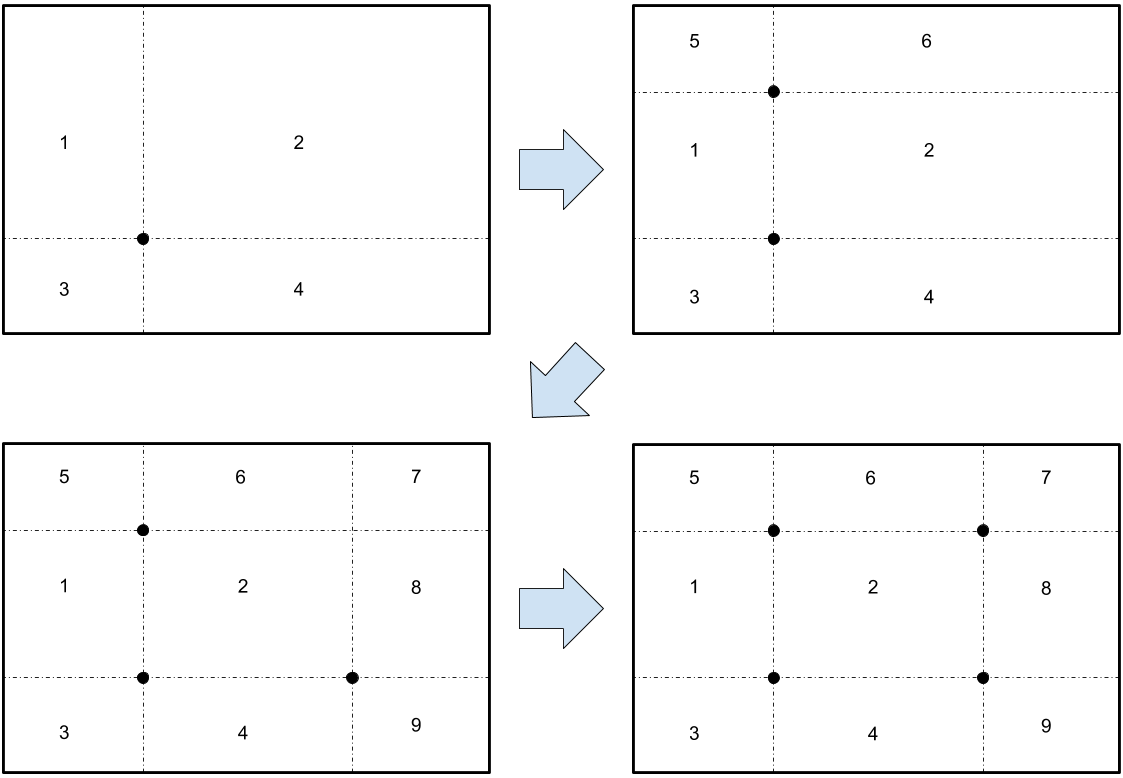
\includegraphics[width=0.85\linewidth]{Separaciones_paredes}
    \caption{Separación de la pared en planos}
    \label{fig:wall_separacion}
\end{figure}

%%%%%%%%%%%%%%%%%%%%%%%%%%%%%%%%%%%%%%%%%%%%%%%%%%%%%%%%%%%%%%%%%%%%%%%%%%%%%
%%%%%%%%%%%%%%%%%%%%%%%%%%%%%%%%%%%%%%%%%%%%%%%%%%%%%%%%%%%%%%%%%%%%%%%%%%%%%
%%%%%%%%%%%%%%%%%%%%%%%%%%%%%%%%%%%%%%%%%%%%%%%%%%%%%%%%%%%%%%%%%%%%%%%%%%%%%

\section{Sistema de estados}
\label{state_pattern}
La aplicación contará con diversos estados principales: vista estándar, vista en planta ortogonal y vista en planta lateral. Cada uno de estos estados tiene propiedades que le diferencian del resto, tienen cámaras distintas y reaccionan de un modo distinto a los inputs del usuario.

La solución más evidente a esto es utilizar un conjunto de condicionales para controlar lo que se hace en cada uno de los estados; pero cuando estos son largos y complejos, el resultado es un código demasiado complicado y difícil de mantener. Además de este modo es fácil cometer errores y que se realicen acciones del estado incorrecto. Para separar mejor cada estado se ha hecho uso del Patrón de Estado\footfullcite{game_programming_patterns}.

Con el Patrón de Estado se define una clase princpial llamada \texttt{Estado}, que define una serie de métodos abstractos: las acciones a realizar para un mismo evento según el estado. En el caso del planificador sus métodos principales son: \texttt{Update}, \texttt{In}, \texttt{Out}, \texttt{OnMouseMove}, \texttt{OnMouseClick}, \texttt{OnMouseDown}, \texttt{OnMouseUp} y \texttt{OnScroll}.

Para los inputs de teclado se ha creado un array de comandos (véase \ref{command_pattern} sobre el Patrón Comando), pudiendo asociar el input con un Comando. Desde la clase \texttt{Estado} se recibe el input de teclado y ejecuta el Comando correspondiente.

La clase \texttt{Estado} debe entonces extenderse mediante herencia, creando otra clase por cada estado que pueda tener la aplicación. Al cambiar entre estados se ejecutará el método \texttt{Out} del estado que cerramos y el método \texttt{In} del que entra. Estos estados son instanciados por ``World" y según el estado actual los inputs y el método \texttt{Update} se redirigen a la instancia correspondiente.

Para que el usuario final pueda cambiar de un estado a otro existirá un input controlado también por ``World".

%%%%%%%%%%%%%%%%%%%%%%%%%%%%%%%%%%%%%%%%%%%%%%%%%%%%%%%%%%%%%%%%%%%%%%%%%%%%%
%%%%%%%%%%%%%%%%%%%%%%%%%%%%%%%%%%%%%%%%%%%%%%%%%%%%%%%%%%%%%%%%%%%%%%%%%%%%%
%%%%%%%%%%%%%%%%%%%%%%%%%%%%%%%%%%%%%%%%%%%%%%%%%%%%%%%%%%%%%%%%%%%%%%%%%%%%%

\section{Gestor de comandos}
\label{command_pattern}
El Patrón de Comandos\footfullcite{game_programming_patterns} permite definir una serie de acciones atómicas. De modo similar a lo que se hace con el Patrón Estado (\ref{state_pattern}) se crea una clase padre llamada \texttt{Comando}. Desde esta clase pueden extenderse comandos que realicen acciones determinadas. Para ejecutar el comando debe crearse una instancia y llamar al método abstracto \texttt{Do} del comando, que se implementa en cada clase derivada.

Este patrón permite implementar la característica de ``deshacer" acciones con el método abstracto \texttt{Undo}. Del mismo modo que definimos una acción por comando podemos definir una contra-acción que deshaga lo hecho. Esto implica que cada vez que se ejecuta la acción debe guardarse el estado previo para poder recuperarlo, si queremos que el comando pueda deshacerse.

Cuando en un comando se ejecuta la acción, su instancia se añade a una lista de acciones realizadas, llamada \texttt{History}. \texttt{History} cuenta con un cursor (un número entero que indica una posición en la lista) que indica la acción en la que se encuentra actualmente, y al deshacer una acción el cursor desciende una posición. Si se desea rehacer una acción, se debe buscar la instancia siguiente al cursor y ejecutar de nuevo su acción.

En el caso de que se realice una acción diferente después de haber deshecho un comando, todos los comandos posteriores al cursor se borran, impidiendo que se puedan rehacer. Se trata sin embargo de un comportamiento habitual de la opción ``deshacer" en otras aplicaciones, por lo que esto no empeora la experiencia de usuario. Si se alcanza el límite de acciones, el historial de acciones empieza a borrar por las primeras posiciones.

Implementar un comando por cada acción posible en la aplicación es sensiblemente más complicado que realizar las acciones sin más, pero este patrón es una de las pocas formas efectivas de implementar la posibilidad de deshacer. Si se decide que es una característica importante para el programa, es importante empezar a utilizarlo desde el principio, puesto que tratar de incluir este patrón en un programa grande y complejo suele requerir una gran inversión de tiempo.

Los comandos se deben instanciar como un puntero, aunque desde fuera no es necesario gestionar su memoria. La implementación utilizada del Patrón Comando registra automáticamente todas las intancias (aunque no estén en el historial) y libera su memoria cuando es necesario.

Otra característica de la implementación utilizada es que puede ejecutarse un comando de forma ``silenciosa" sin que este se registre en el historial, mediante el método \texttt{Do\_Silent}. Entre otras cosas, esto puede utilizarse para deshacer acciones aprovechando otros comandos existentes: si por ejemplo tenemos la acción ``añadir" y ``borrar", el método \texttt{Undo} de cada uno de ellos puede hacerse con una llamada silenciosa al otro. Esto ahorra complejidad y, si un comando cambia, no es necesario buscar sus equivalentes por el código para reflejar los cambios.

La implementación de cada comando queda como responsabilidad del usuario, en el apartado \ref{use_of_command} se dan detalles del uso que se le ha dado al patrón.

%%%%%%%%%%%%%%%%%%%%%%%%%%%%%%%%%%%%%%%%%%%%%%%%%%%%%%%%%%%%%%%%%%%%%%%%%%%%%
%%%%%%%%%%%%%%%%%%%%%%%%%%%%%%%%%%%%%%%%%%%%%%%%%%%%%%%%%%%%%%%%%%%%%%%%%%%%%
%%%%%%%%%%%%%%%%%%%%%%%%%%%%%%%%%%%%%%%%%%%%%%%%%%%%%%%%%%%%%%%%%%%%%%%%%%%%%

\section{Clases contra espacios de nombre}
Una decisión importante de diseño ha sido la de no utilizar en ningún caso el patrón Singleton. El patrón Singleton limita a una la cantidad de instancias que se puede tener de la clase que lo aplica, lo cual impide que se haga un mal uso de la clase si su propósito era que fuese una clase de una única instancia. Para conseguirlo se hace que el constructor de la clase sea privado y que la clase tenga una referencia estática y privada de sí misma dentro; el Singleton se encarga de manejar su propia instancia.

Aunque es un patrón muy útil y sencillo, en la mayoría de casos puede resolverse el problema de un modo más simple, como utilizando una clase que solo tenga métodos estáticos o, en C++, con funciones dentro de espacios de nombre. Un espacio de nombre es un ámbito (más conocido como scope) que permite limitar el acceso a su contenido, no se puede llamar a ninguna de sus funciones ni acceder a sus variables si no se especifica antes su espacio de nombre. Desde fuera, puede utilizarse del mismo modo que se haría con una clase puramente estática, pero tiene algunas diferencias importantes:

\begin{itemize}
    \item Puede extenderse y definirse en ficheros distintos. Es algo que ayuda a la mantenibilidad si el código es extenso y complejo, puesto que es posible separar las diferentes partes. Por otro lado, una desventaja es que el programador usuario del espacio de nombre también podría definir lo que quisiera dentro de este, abriendo la puerta a ``hacks", aunque en estos casos se asume que la responsabilidad es de quien utiliza mal la herramienta.
    
    \item No tiene métodos ni atributos privados. Sin embargo, es posible emular el comportamiento de los elementos privados extendiendo la clase dentro de la especificación del código, ocultándolo por tanto de los ficheros de cabecera, que son los que permiten que un código sea accesible desde otros puntos del programa.
    
    \item No tiene herencia. No es posible utilizar herencia en espacios de nombre, es una característica única de las clases. Si la herencia es importante los espacios de nombre quedan descartados.
\end{itemize}

Otro de los beneficios de un espacio de nombre es que permite evitar colisiones de nombre entre funciones y variables. Por ejemplo, si una de las librerías utilizadas tuviera una función llamada ``max", sería posible redefinirla dentro de un espacio de nombre.

Al final se ha escogido esta opción como sustituto del patrón Singleton en todos los casos donde no se requiera herencia ni instancias.
